\chapter{Object reconstruction and identification}
\minitoc
The form of the raw data collected by the CMS detector is in detector hits and deposited charge information. Therefore, it is not suitable to be used directly in the physics analyses.\\
In this chapter the reconstruction and identification of physics objects used in the CMS experiment is discoursed.
These objects and their kinematic characteristics are used in building the event selection criteria which will be discussed in Chapter \ref{Chap:eventSel}.
\section{Particle-Flow algorithm}
\label{sec:PF}
Figure \ref{fig:CMS_Slice} displays the trails of the particles passing trough the sub-detectors of CMS experiment. Only energy deposits in the most relevant sub-detectors are presented otherwise a particle can leave trace in multiple detector layers. The particle-flow (PF) algorithm \cite{PF,PF2}, uses the information obtained from the all detector subsystems in the object reconstruction. Three main features of the CMS PF algorithm are tracks reconstructed from hits in the tracker, energy deposits in the calorimeters and tracks reconstructed from hits in the muon system. In order to archive object reconstruction with a high efficiency and low fake rate, iterative tracking and the calorimeter clustering methods are used in the PF algorithm. The Kalman filter \cite{KalmanFilt} method, which ensures a proper track finding even for objects with low $\pt$, is adopted to identify single particle tracks. Calorimeter clustering is responsible for several tasks such as the detection and measurement of stable neutral particles, their isolation from charged objects, reconstruction and identification of electrons and corresponding Bremsstrahlung photons.After determining the single elements, a linking algorithm is used to form a block from separate elements that are possibly related to a single object. After the construction of blocks, the actual particle reconstruction and identification is performed. The objects are reconstructed in a squence of highest reconstruction performance to lowest, thus already identified blocks are gradually discarded for the more ambiguous object reconstructions. \\
For muons, the tracks in the muon system is fit to the inner tracks by requiring an acceptable $\chi^2$. These muons are also called global muons. If the momentum of a global muon is compatible with the tracker-only measurement within three standard deviations, a particle-flow muon is formed. \\
Generally, an electron goes into a bremsstrahlung radiation, which results in a more complicated reconstruction procedure than the muons. Gaussian sum filter \cite{GSF} algorithm which also accounts for the possible energy loses is used to perform the track fitting. Moreover, a second algorithm based on ECAL superclusters determines the electromagnetic energy deposits that are aligned to electron candidate tracks. A particle-flow electron is formed, if the track-cluster compatibility is satisfied.\\
At this point, after removing the identified muons and electrons tracks, the neutral and charged hadrons are reconstructed from the remaining tracks and the matching calorimeter deposits. The reconstruction for photons and $\tau$-leptons will not be described since they are not used in this analysis. Detailed discription of these objects can be found here \cite{Photon1}. \\
In this analysis, the kinematic variables, which are introduced in Chapter \ref{Chap:eventSel}, are based on the reconstructed objects satisfying certain identification criteria.
\begin{figure}
\begin{center}
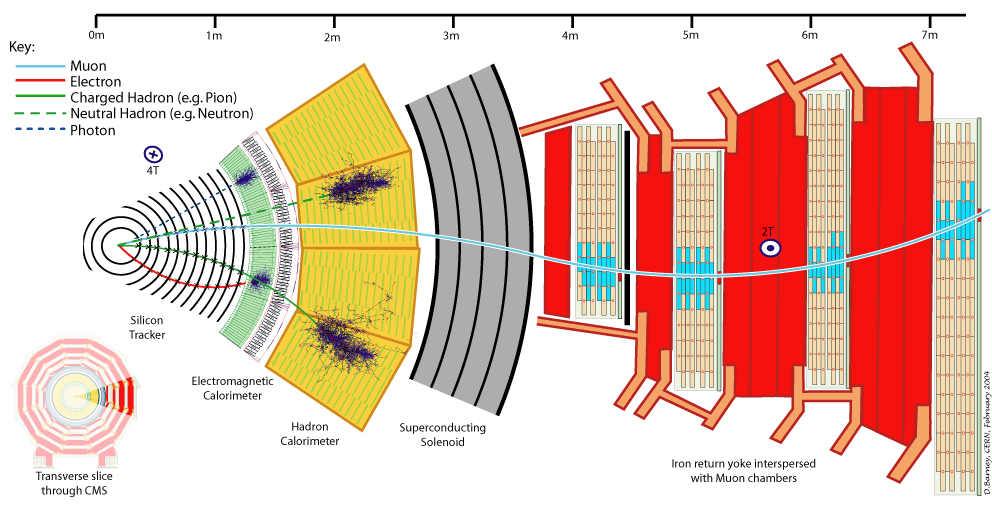
\includegraphics[width=\textwidth]{Plots/CMS/CMS_Slice}
\caption{\label{fig:CMS_Slice} Cross section of a slice of the CMS detector in the transverse plane with different particles crossing the subsystems is shown \cite{CMS_slice}. Only energy deposits in the most relevant subdetectors are presented for simplicity.}
\end{center}
\end{figure}
%\newpage
\section{Physics Object reconstruction and identification}
\subsection{Primary vertices}
\label{sec:PV}
To describe an event, the primary vertex (PV) is the main quantity. The primary vertex is where the interesting parton collision takes place.\\
The very high instantaneous luminosities of the LHC results in a quite high probability of multiple proton-proton interactions per bunch crossing, pile-up. Therefore, a precise reconstruction of PV is a challenging task.\\
The reconstruction commences with selecting a set of tracks based on some quality criteria such as the number of hits in the tracker and the impact parameter. Next, the selected tracks are clustered according to their z-coordinate. A vertex fit \cite{VertFit} is then applied on the clusters that more than 1cm apart and contain at least two tracks. Finally, the primary vertex of interest is chosen to be the cluster with the largest sum of the squared track momenta.\\
A vertex is assigned as good if the number of degrees of freedom of the fit result is larger than four. In the present analysis, at least a good primary vertex is required in the event selection.
%\newpage
\subsection{Leptons}
In the context of this thesis, only the events with single lepton are considered; therefore lepton reconstruction and identification has a great importance. Additional requirements on the particle flow leptons are applied to ensure choosing a good quality lepton or rejecting the fake ones.\\
In this analysis, only the leptons in the acceptance of $|\eta|<2.4$ with a transverse momentum of $\pt>$10 GeV are considered.
\subsubsection{Muons}
First, the muons are defined as good if they satisfy several CMS-wide identification criteria. A candidate is a good muon if the fraction of valid tracker hits above eighty percent. Furthermore, several conditions are imposed according the segment compatibility evaluation. The segment compatibility is used to quantify the compatibility of a tracker-muon object with the muon hypothesis \cite{segment}. If the segment compatibility computation returns a value larger than 0.451 then the muon is selected, otherwise if it is below 0.303 the muon is rejected. For the candidates with intermediate segment compatibility further requirements are levied: the muon is a global muon, the global fit gives a $\chi^2$ less than three, the $\chi^2$ of the matching between the tracker and muon is below twelve and the value returned by the kink finder is below twenty. \\
In addition to CMS-wide identification selections, several criteria specific to this analysis are also applied. Two types of muons are defined as tight and loose. The loose muons are required to have a mini isolation \cite{miniIso}, for which an explanation can be found following to this paragraph, less than 0.4. The candidates with $\pt>$25 GeV, the mini isolation less than 0.2 and have the three-dimensional impact parameter significance less than four are defined as tight muons. \\ 
In this search, only events with one tight muon and no other loose muons are considered if the lepton is not electron.
The isolation of a lepton is a measure of the relative additional activity in a predefined lepton cone. For a more analysis specific selection, a varying cone radius is selected according to the $\pt$ of the lepton. For a lepton coming from a boosted $W$ boson, which then will have a high $\pt$, a narrower cone size is chosen. More precisely, cone radius is set to 0.05 for the leptons with $\pt\geq$200 GeV, while for the leptons have $\pt$ less than 50 GeV a larger cone radius of 0.2 is considered. For the leptons with intermediate $\pt$, con size is given by the formula: $\frac{10\,GeV}{p_{T,\,lep}} $.
The mini isolation is also used for the electron selection for which the criteria will be given in the following.
\subsubsection{Electrons}
As mentioned earlier the particle flow reconstruction of good quality electrons \cite{ELEID} is more elaborate than the muons. 
Similarly to the muons case, a list of CMS-wide identification requirements are imposed on the particle flow electrons identified by using Gaussian sum filter. The list of criteria with short descriptions is given in Tab. \ref{tab:EleSel}. The requirements are slightly changing between the Barrel and the Endcap regions, due to the different granularity of ECAL. Those criteria \cite{ELEID2} in the list involve the shower shape quality and the cluster energy and track momentum compatibility. In addition to the list no associated photon conversion vertex is required.\\
On top of the CMS-wide identifications also analysis specific selection criteria is also applied. In the electron case, leptons with $\pt>25$GeV and with mini isolation smaller than 0.1 are defined as tight. For electrons, due to the identification inefficiency in the overlapping region between the ECAL barrel and endcaps, the corresponding pseudorapidity region $1.44<|\eta|<1.56$ is excluded. The number of leptons fail to satify these criteria is set to be zero if the lepton is not muon.\\  
\renewcommand{\arraystretch}{1.5}
\begin{table}[ht]
\begin{center}
\begin{tabular}{|c|l|c|c|}\hline
Selection        & Definition & Barrel & Endcap \\
\hline
\hline
$\sigma_{i\eta i\eta}$& ECAL crystal-based shower covariance in the direction of $\eta$& 0.0101&0.0283\\\hline
$\Delta\eta_{in}$ &Difference between the supercluster position in the ECAL & 0.00926& 0.00724 \\
& and the track direction at the innermost tracker position in $\eta$&&\\\hline
$\Delta\phi_{in}$ &Difference between the supercluster position in the ECAL &0.0336 &0.0918\\
 & and the track direction at the innermost tracker position in $\phi$  & &\\\hline
H/E & Ratio of energy measured in the HCAL over&0.0597&0.0615\\
& the energy mea- sured in the ECAL&&\\\hline
$|1/E \, -\,1/p |$& Absolute difference between the inverse electron energy&& \\
&measured in the ECAL and the inverse momentum &0.012&0.00999 \\
&measured in the tracker && \\\hline
$\Delta_{xy}$&Track-vertex distance in the transverse plane &0.0111&0.0351\\\hline
$\Delta_{z}$& Track-vertex distance along the beam axis&0.0466&0.417 \\\hline
$N^{miss}_{hits}$&Number of missing hits in the electron inner layer track& $\leq2$&$\leq1$\\\hline
\end{tabular}
\end{center}
\caption{List of selection criteria for the CMS electron identification.}\label{tab:EleSel}
\end{table}
\renewcommand{\arraystretch}{1}
\subsection{Jets}
\label{sec:PFJET}
In the context of this thesis, in the decays of supersymmetric gluinos, an abundance of jets is expected in the final state.\\
As already briefly mentioned in Sec.\ref{sec:StandardModelParticleInteractions}, cascade decays of quarks and gluons leads to a collimated spray of hadrons. In experiments, this signature is also known as jet. 
As jets of particles propagate through the CMS detector, according to their particle content, they leave traces in all of the sub-detectors. To form a reconstructed jet, all these detector responses are combined using various jet algorithms.  
In CMS there are two types of jet clustering algorithms in use: Cone algorithms and sequential algorithms. The first one uses a geometrical shape assumption, while the latter starts with clustering two of the closest objects together and iteratively reconstruct a closed area of objects until a truncation criterion is satisfied \cite{JET1}.\\
The distance used as the termination criterion can be formulated in generalised form as:
\begin{eqnarray}
{d_{i,\,j} =  min\,(k^{2p}_{{\rm t},i},k^{2p}_{{\rm t},j})\frac{\Delta^2_{i,\,j}}{R^2}}\,,\\
{d_{i,\,B}} = k^{2p}_{{\rm t},i}\,,
\end{eqnarray}
where $d_{i,\,j}$ represents the distance between entities (particles, pseudojets) $i$ and $j$ and $d_{i,\,B}$ is for the distance between the entity $i$ and the beam ($B$). In the formula, $\Delta^2_{i,\,j}$ is the spatial distance in $y-\phi$ plane and $k_{{\rm t},i}$ is the transverse momentum. The $d_{i,\,j}$ is calculated iteratively until it is $d_{i,\,B}$ and then i is called a jet and it is removed from the list of entities. According to different values of $p$, which is governing the relative power of the energy versus geometrical ($\Delta_{i,\,j}$) scales, three main algorithms can be defined.\\
The case of $p=0$ corresponds to the Cambridge/Aachen algorithm where the termination condition is described by purely geometrical distance. The $p=1$ case is called the ${\rm k_t}$ algorithm which involves the transverse momenta of the entites as well as the geometrical distance parameter. \\
In this analysis, the anti-${\rm k_t}$ algorithm, which is the case of $p=-1$, is used to cluster the particle flow candidates into jets. For the curious readers, the anti-${\rm k_t}$ algorithm and its performance in comparison to other algorithms are explained here \cite{antiKT}.\\
In the present search, particle flow candidates are clustered into $R = 0.4$ jets. Jets are required to be within the pseudo rapidity range of $|\eta|<$2.4 which corresponds to the tracker acceptance. Moreover, if the energy fraction of one of the components such as the neutral, charged electromagnetic or hadronic exceeds 99\% then the jet is rejected.\\
The main purpose of the algorithm is to reproduce the energy of the original parton prior to the shower. However, the measured jet energy is not the same as the corresponding parton. There are several reasons such as the non-uniform detector response, electronic noise responsible for this difference. In CMS, these effects mostly covered with Jet Energy Calibrations (JEC) \cite{JEC}.\\
In this search, after all corrections are applied to a reconstructed jet, the transverse momentum is required to be larger than 30 GeV.
%Next, the corrections, which are known as Jet-Energy Corrections can be applied to the measured energies \cite{JEC}.
%The algorithm aims to reproduce the energy of the original parton prior to the shower.
\subsection{b tagged Jets}
\label{sec:btagging}
For many SM and new physics processes, jets, which are originating from b quarks, are important since a number of these processes involve top quark decays. However, in the present analysis, the targeted SUSY model T5qqqqWW (see Sec.\ref{sec:simplifiedModels}), involves no top quark; therefore in the final state no jets coming from b quarks is expected. In the analysis, the events including b quark tagged jets are used to perform the $\ttJets$ background estimation (see Sec.\ref{sec:RcsTT}).
\\
Thus, the identification of jets coming from b-quark hadronization, which is also referred as b-tagging, is an important task.
Generally, the identification technics \cite{btagging} utilize the rather long lifetime and high mass of the b quark which leads to a displaced vertex formation.\\
A variety of algorithms have been developed by CMS \cite{btagging2} to select b-tagged jets based on the variables such as the impact parameters of charged-particle tracks, the assets of reconstructed decay vertices, and the presence or absence of a lepton or combination of some of them. Each of these algorithms results in a single discriminator value for each jet. 
In this analysis, the combined secondary vertex (CSV) algorithm is employed with medium working point (0.8484), which corresponds to a tagging efficiency of about 70\% and a misidentification rate of about 1\% accordingly to the $\pt$ and $\eta$ of the jet.\\
The possible differences between the performance of the b-tagging algorithm measured in data and in simulation are compensated by applying scale factors to simulated events, the basic principles are mentioned in Sec.\ref{sec:SF}.
%To identify the b-tagged jets, naturally, the first step is to determine those secondary vertices (SV). 
%mention fake rate 
%\newpage
\subsection{Missing transverse energy}
One of the main purposes of the present search is to investigate the potential discovery of SUSY models, which involve dark matter candidates such as neutralinos in the form of the lightest stable supersymmetric particle. However, these particles as well as the weakly interacting SM neutrinos are invisible in the CMS detector in other words they don’t leave any trace in the subsystem. Only imbalance in energy and momentum can be a hint for their existence. The momentum imbalance in the transfers plane is called missing transverse energy and its vector form is denoted as $\METvec$ while the magnitude is $\MET$. Therefore, $\METvec$ can be formulated as the negative vector sum of the transverse momentum $\pt$ of all observed particles:
 \begin{eqnarray}
 \label{Eqn:MET}
{\METvec =  -\sum_i\ptveci}\,,
\end{eqnarray}
where the index $i$ iterates over all particle flow candidates, which are associated with the primary vertex, to calculate the particle flow $\MET$, $PF-\MET$. Otherwise, the case where $i$ stands for the calorimeter deposits is a another $\MET$ type used in CMS which is known as $Calo-\MET$. A third type of $\MET$ is an improved version of $Calo-\MET$ by corrections obtained from the tracking detector and it is called $TC-\MET$.
Naturally, as it can be understood from the name, $PF-\MET$ is reconstructed by using the particle flow algorithm \cite{MET}. \\
In the CMS detector, a momentum imbalance can be also originated through the various subdetector malfunctions, reconstruction effects. \\
%To be able to determine the amount of this $fake-\MET$, generally DY events where a Z boson decays to two opposite sign leptons are used because of the fact that in these kind of events the expected $real-\MET$ contribution is very low. In data, these events are selected by requiring the invariant mass of the dimuon or dielectron system is inside the Z-boson mass window, 60GeV$<M_{\ell\ell}<$120GeV.\\
The mis-calculation of $\MET$ due to the possible reconstruction problems of PF particles can be reduced by propagating the aforementioned jet energy corrections to the $\MET$ calculation.
In CMS, particles generally are produced uniformly in $\phi$, thus $\METvec$ is expected to be independent of $\phi$. However, due to the $\phi$-dependence of the detector response, imperfect alignment of different detector subsystems, or a $\sim4$~mm shift between the centre of the detector and beamline \cite{CMS-PAS-TRK-10-003}, an asymmetry in $\phi$ is observed in data and in simulated events.\\
The observed $\phi$-asymmetry can also be explained by a shift in the $\METvec$ components along the x and y detector axes, which are denoted as $\mex$ and $\mey$ respectively. The shift shows a linearly increasing trend as a function of multiplicity of the PF candidates. To obtain the corrections, this correlation is used. First, linear fits are performed on $\mex$ and $\mey$ distributions as a function of number of PF candidates in various $\eta$ bins. Examples of these fits are shown in Fig. \ref{fig:phiFits}, where the linear dependence of $\langle\mex\rangle$ and $\langle\mey\rangle$ 
on multiplicity of PF candidates can be formulated as:
\begin{eqnarray}
\left<\mex \right> & = & c_{x_o} \cdot x + c_{x_s} \cdot x^2, \nonumber \\
\left<\mey \right> & = & c_{y_o} \cdot x + c_{y_s} \cdot x^2.
\label{eq:metPhiAsymmetryFitModel}
\end{eqnarray}
\begin{figure}[!h]
\begin{center}
\subfigure[$\mex$, number of gamma]{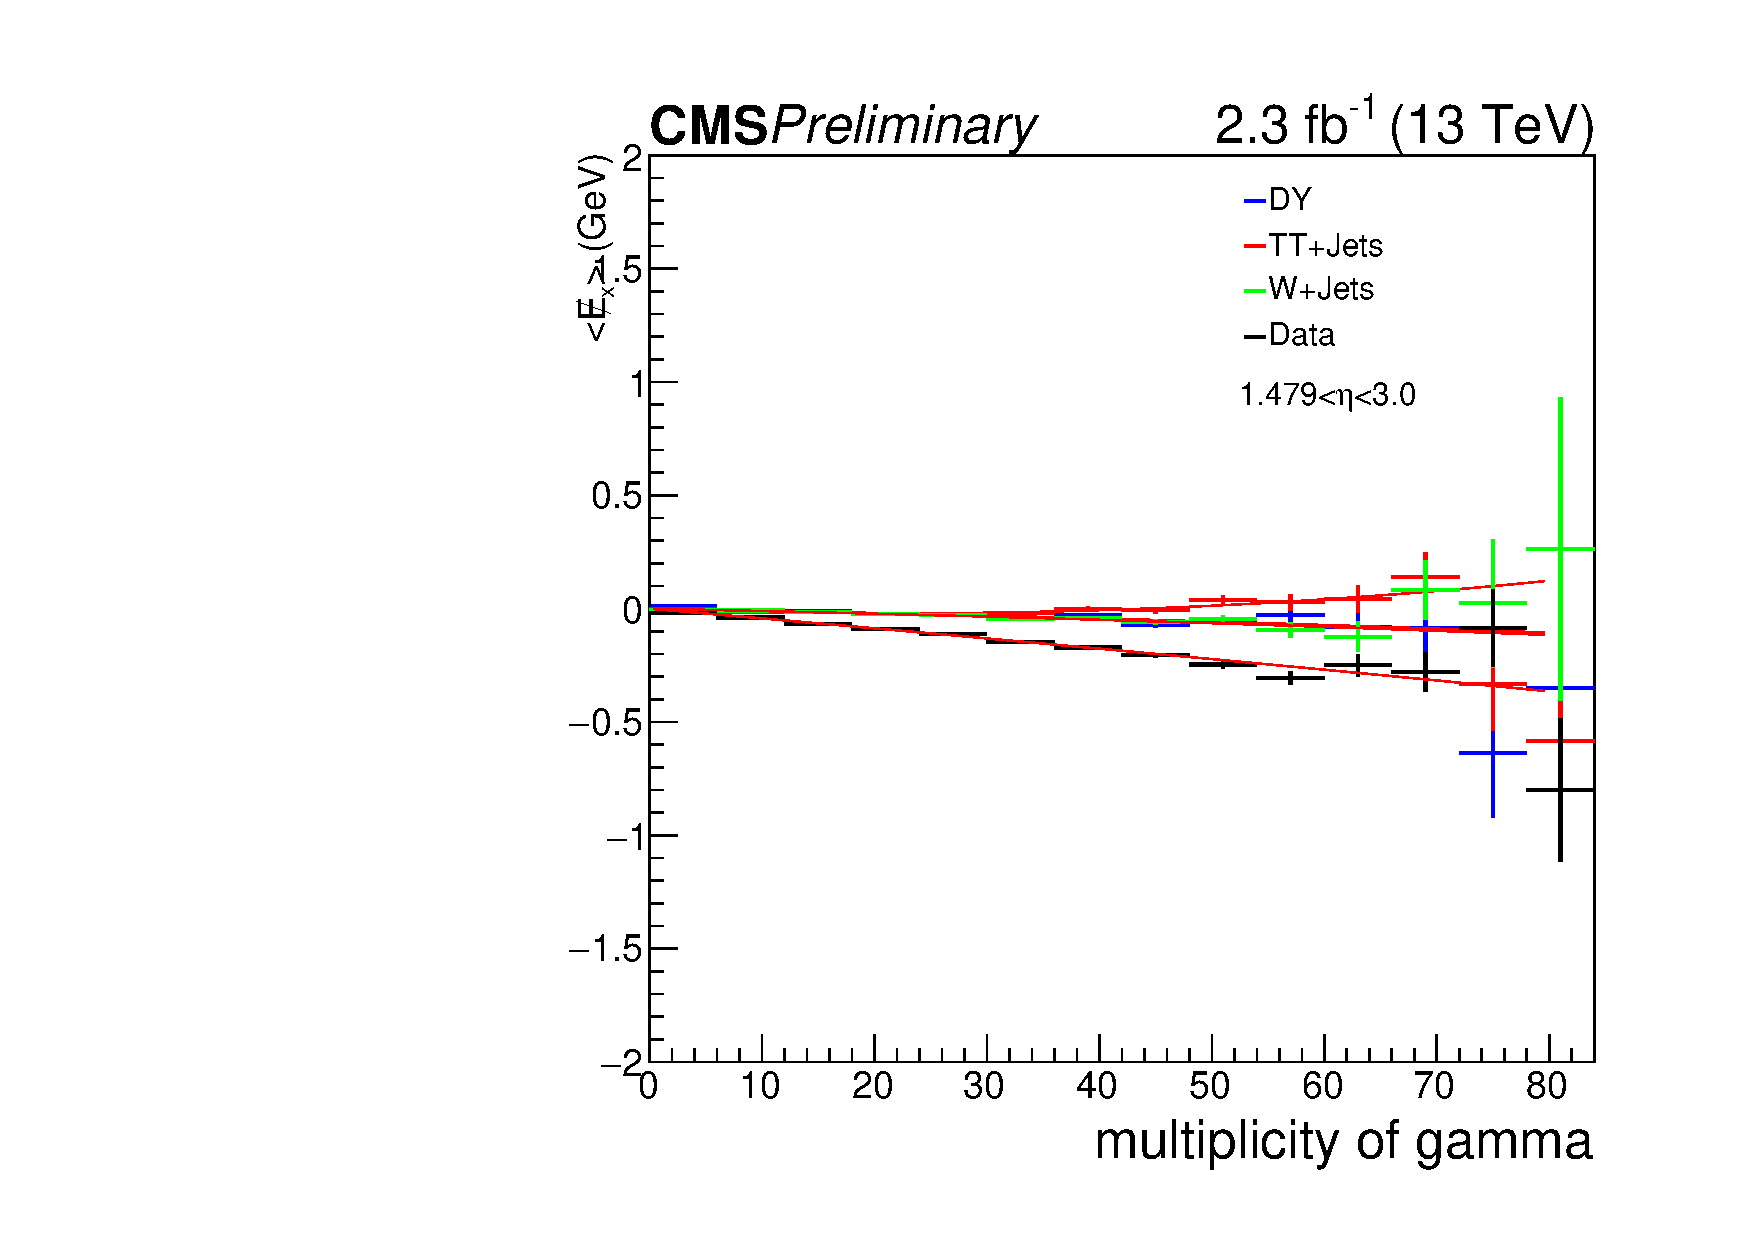
\includegraphics[width=0.35 \textwidth]{Plots/metphi/gammaEndcapPlus_Px_mult_withData_zoomedIn_PAS.pdf}}
\subfigure[$\mey$, number of gamma]{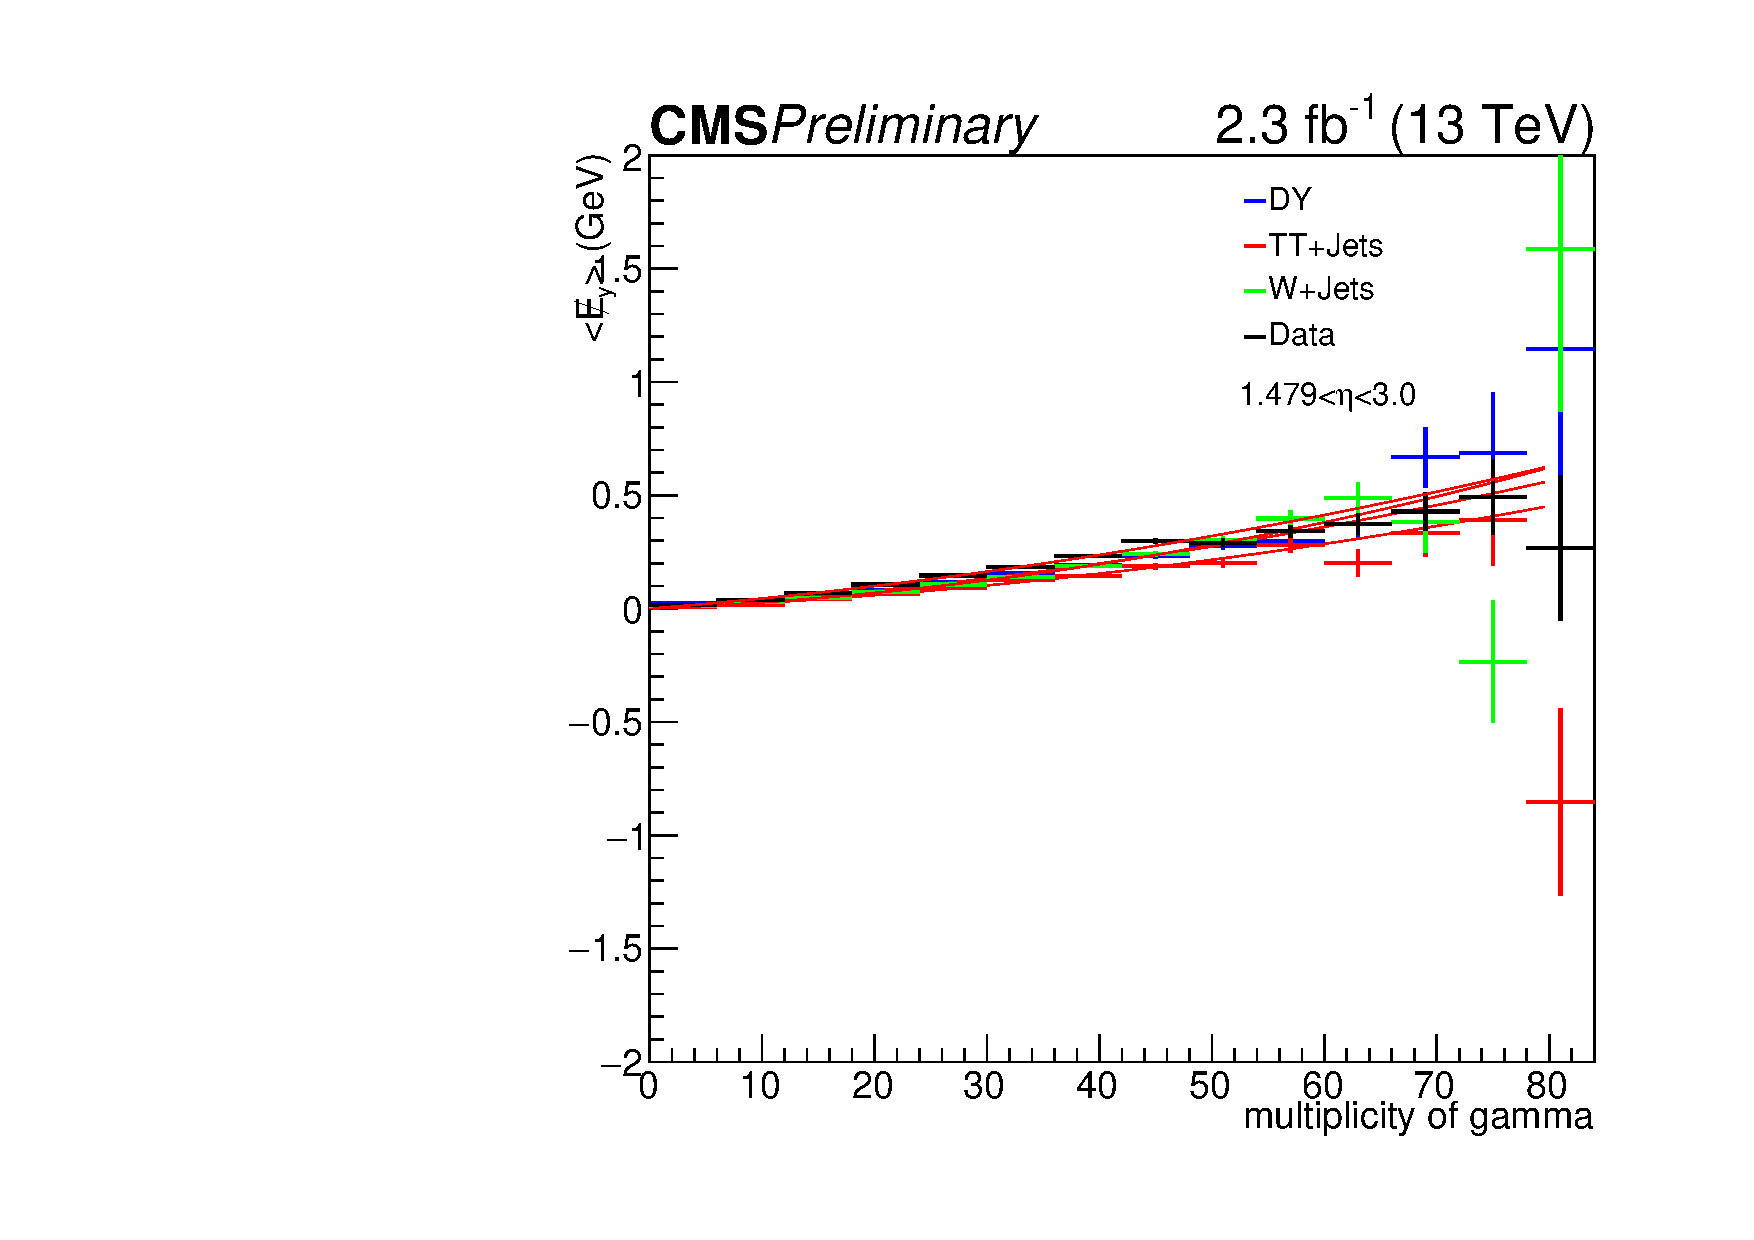
\includegraphics[width=0.35 \textwidth]{Plots/metphi/gammaEndcapPlus_Py_mult_withData_zoomedIn_PAS.pdf}} \\
\subfigure[$\mex$, number of neutral hadrons]{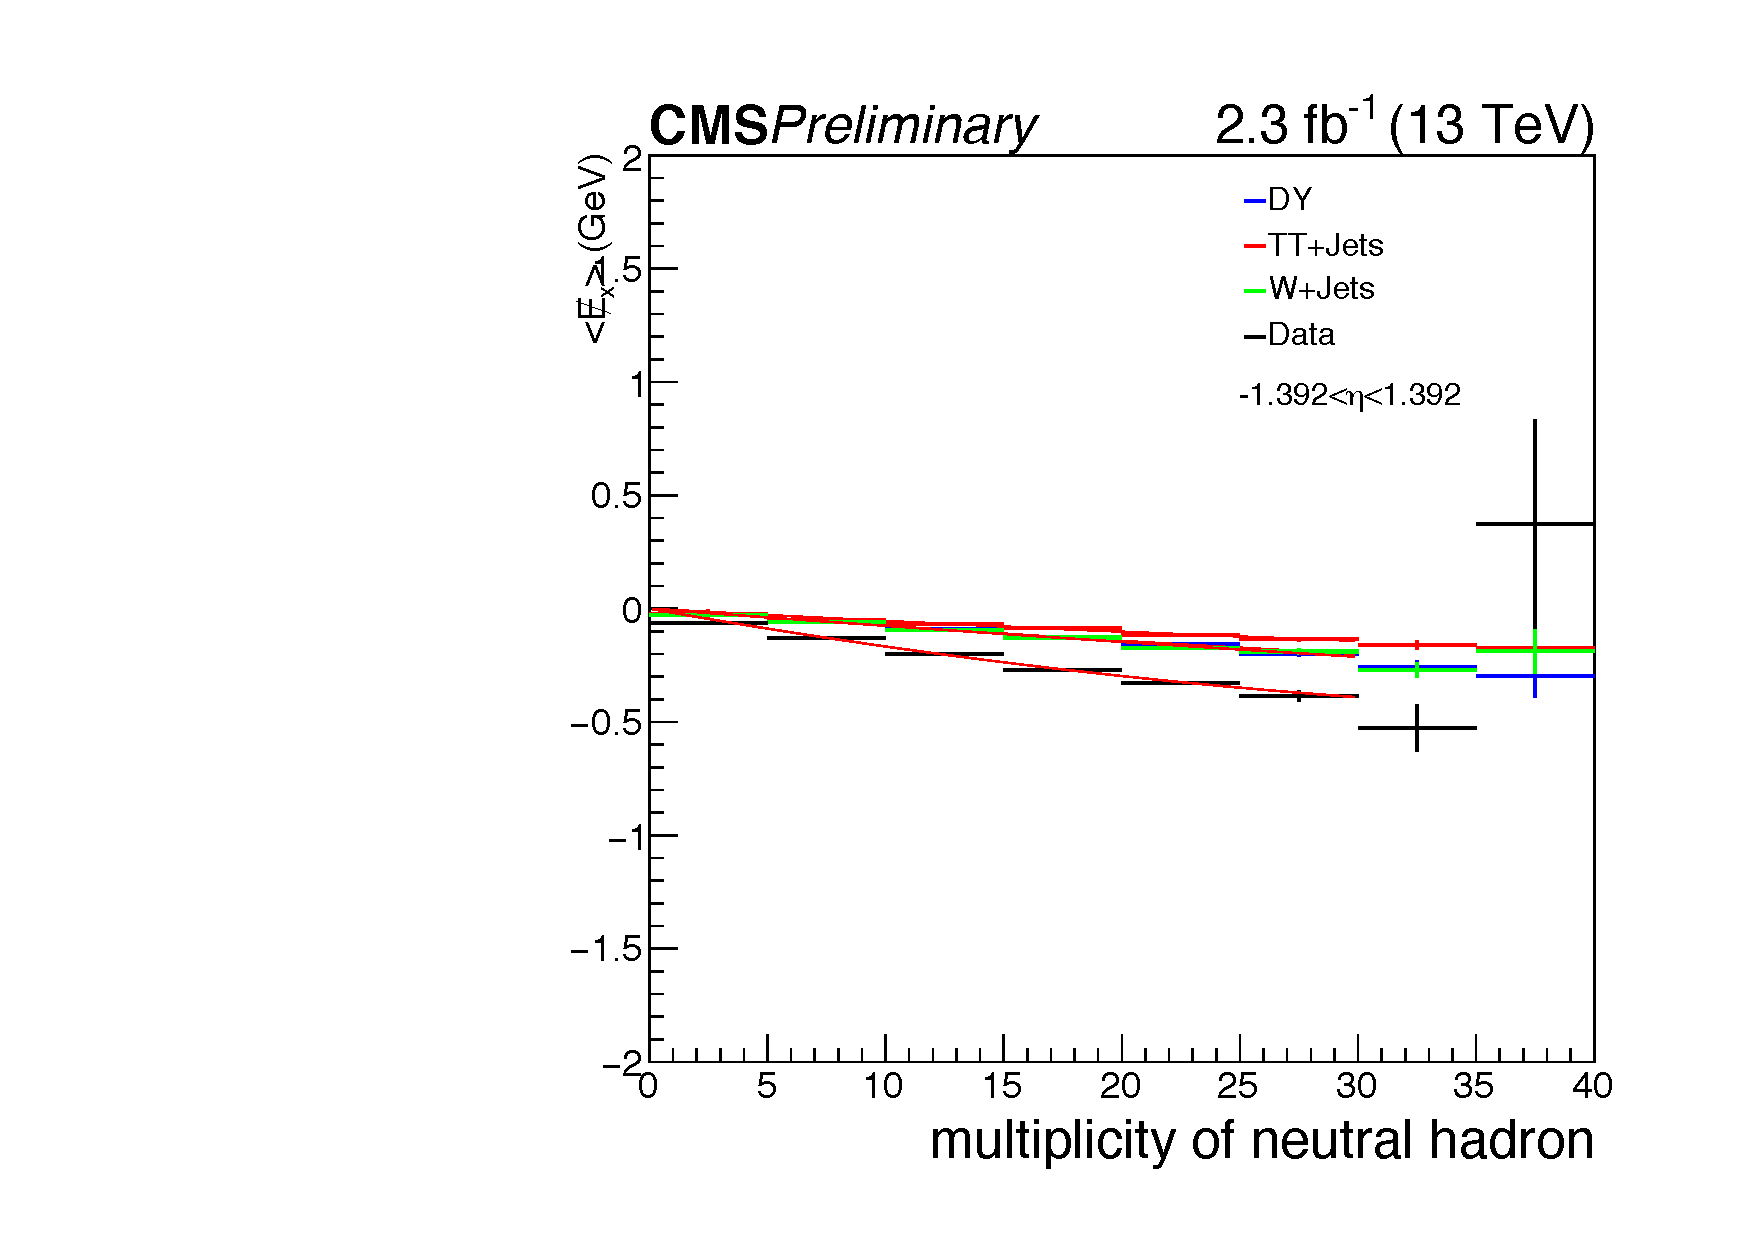
\includegraphics[width=0.35 \textwidth]{Plots/metphi/h0Barrel_Px_mult_withData_zoomedIn_PAS.pdf}}
\subfigure[$\mey$, number of neutral hadrons]{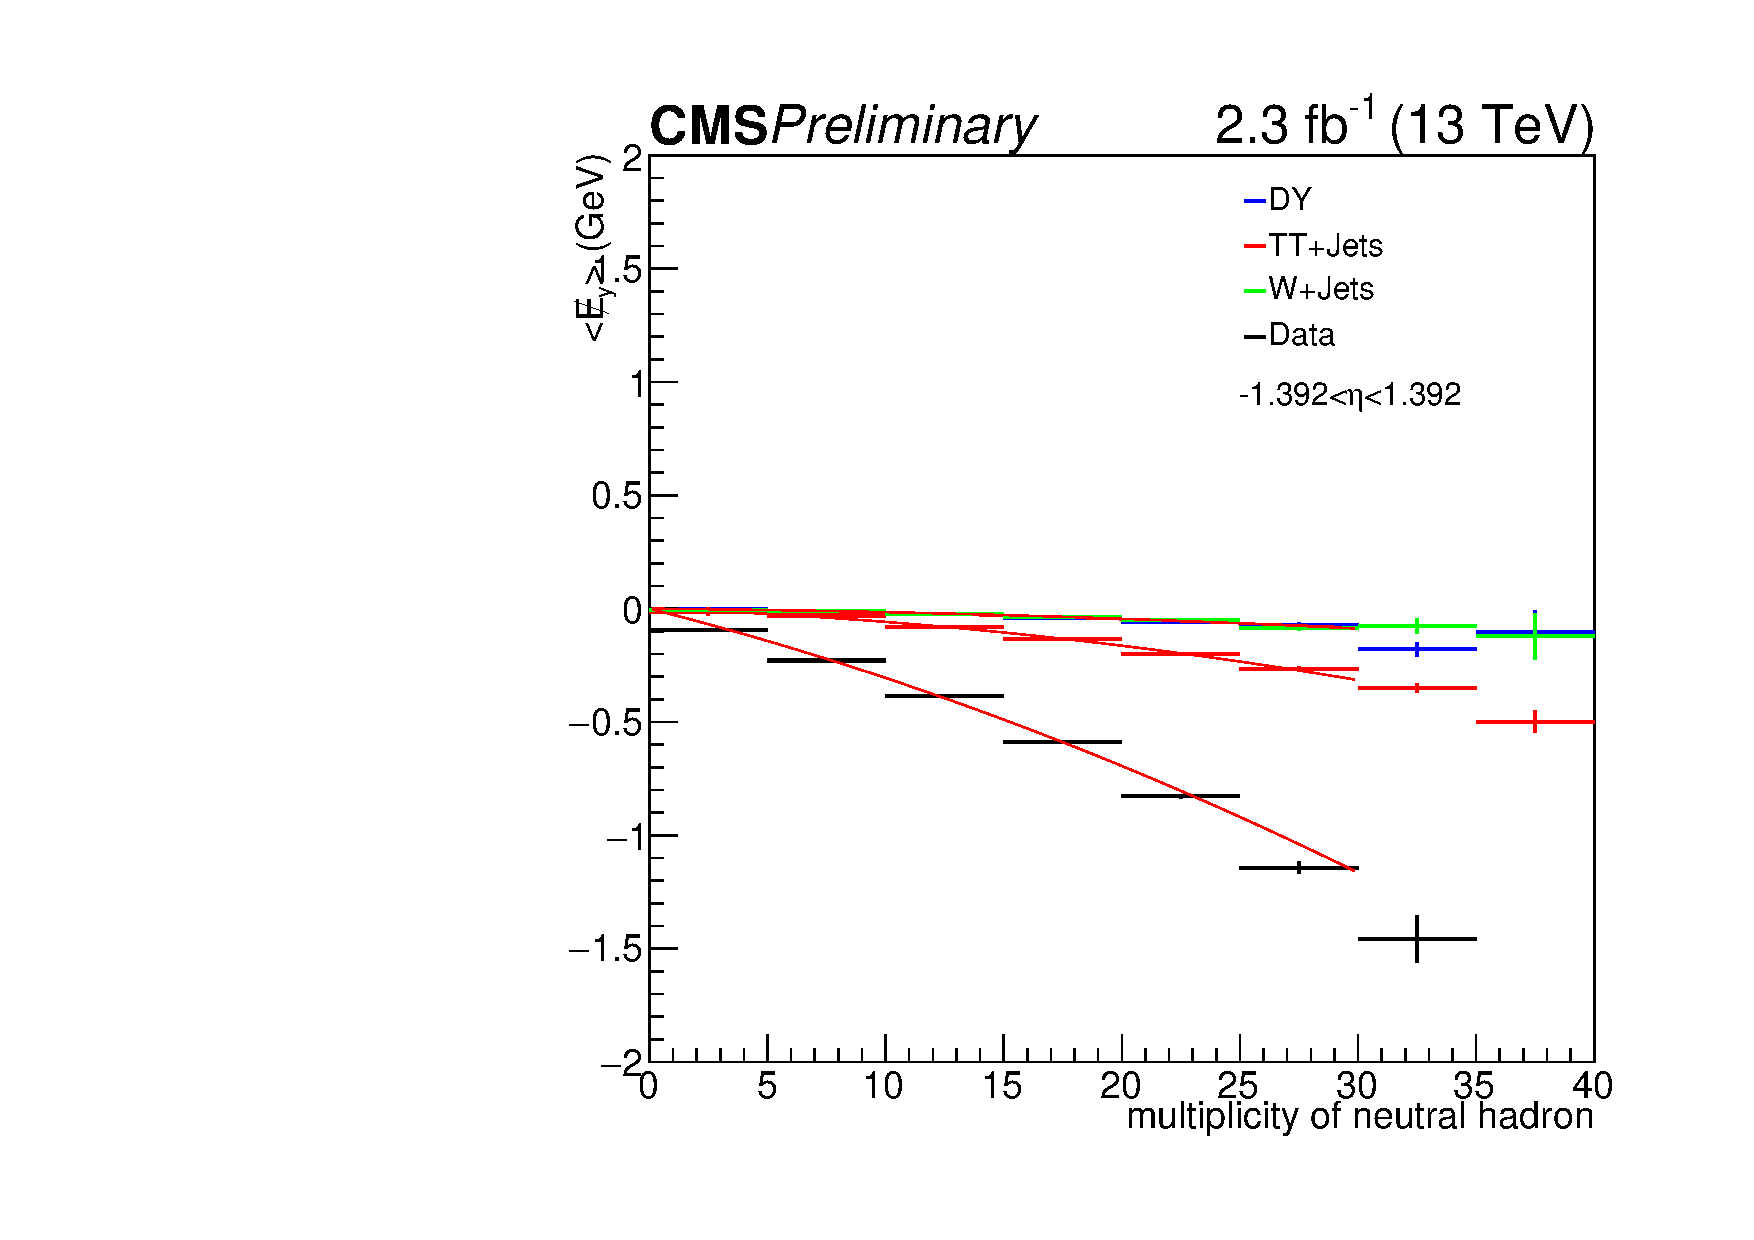
\includegraphics[width=0.35 \textwidth]{Plots/metphi/h0Barrel_Py_mult_withData_zoomedIn_PAS.pdf}} \\
\caption{
  PF candidate multiplicity fits for \mex and \mey in different $\eta$ regions.
  }\label{fig:phiFits}
\end{center}
\end{figure}
After the fits are performed, the corrected $\mex$ and $\mey$ can be obtained on an event-by-event basis as:
\begin{eqnarray}
\mex^\mathrm{corr} &=&  \mex - \left<\mex \right>= \mex  -(c_{x_o} \cdot x + c_{x_s} \cdot x^2), \nonumber \\
\mey^\mathrm{corr} &=&  \mey - \left<\mey \right> = \mey -(c_{y_o} \cdot x + c_{y_s} \cdot x^2).
\end{eqnarray}
The coefficients $c_{x_0}$, $c_{x_s}$, $c_{y_0}$, and $c_{y_s}$ are determined
separately from data and simulated samples. In simulated samples, the corrections are obtained by using DY events where a $Z$ boson decays to two opposite charged leptons. In these kind of events the expected $real-\MET$ contribution is very low, thus they provide a very good environment to measure $\MET$ mismodelings. The validation of the procedure is performed by using $\ttJets$ and $\wJets$ simulated samples. In data, the corrections are obtained in events with the invariant mass of the dimuon or dielectron system is inside the Z-boson mass window, 60GeV$<M_{\ell\ell}<$120GeV.
%\newpage
